%{\normalfont\initfamily \fontsize{12mm}{12mm}\selectfont D}
\begin{multicols}{2}

 
  \cappar Estimados lectores de nuestra revista, en este último número
  de nuestro primer año en la revista me he permitido escribir este
  artículo para contaros con un poco detalle como se está haciendo la
  historia de esta revista. Me llamo María y soy la coordinadora de la
  revista. Hace poco más de un año la empresa Saema me ofreció
  colaborar en la creación de una revista científica--divulgativa
  donde tuviésemos la oportunidad de mostrar como las matemáticas son
  una herramienta hermosa en temas de ingeniería, especialmente en
  temas de energía y aguas que es donde son especialistas la empresa
  Saema. Cuando yo comencé ya estaba nuestro compañero Bartlomiej
  Skorulski, también doctor en matemáticas, montando el diseño de la
  revista y escribiendo los primeros artículos sobre la
  catenaria. Estábamos emocionados de participar en un proyecto donde
  nuestro principal objetivo era daros, a vosotros, nuestros lectores,
  una buena calidad de información.

  Como sabéis a día de hoy nuestra revista tiene varias secciones. La
  primera sección la llamamos \emph{Nada es Imposible} y hoy me he
  colado yo en ella. Esta sección quería que, vosotros y a veces
  nosotros, hablásemos de nuestra experiencia con las ciencias, de
  como vemos las ciencias en Ángola y sobre todo de hacer ver que no
  hay nada imposible que no se pueda hacer con fuerza e ilusión. La
  segunda sección titulada \emph{Solución en acción} estaba destinada
  a gente que hace posible que hoy Saema esté aquí. Hemos recorrido
  por varias experiencias de trabajadores de Saema y de amigos de
  Saema contándonos su día a dia y mandando mensajes al pueblo
  angolano. La sección de Matemáticas en ingeniería es el corazón de
  la revista. Es propiamente lo que más la define e intentamos
  explicaros y acercaros a las matemáticas escritas entre postes de
  luz, entre tuberías y entre ondas de una buena música como la de
  Bonga. La sección de \emph{Informática en Ingeniería} la pensamos
  porque cada vez es más importante en estas décadas tener algunos
  conocimientos de informática que te den posibilidad para poder crear
  aquellas cosas que pueden rondar en tu cabeza. La programación está
  inmersa en el día a día y hacerte partícipe de ella para entender
  mejor el mundo creemos es importante. Este primer año nos hemos
  dedicado a un lenguaje funcional y muy potente que es Octave. Espero
  lo hayas disfrutado y hayas podido seguir las diferentes
  prácticas. En este último número del año te damos varios problemas
  pra desarrollar con Octave. ¡Disfrútalos!  En la sección de
  \emph{Novedades} os contamos algunas curiosidades que hemos pensado eran
  dignas de dedicarles un artículo para compartir con todos
  vosotros. Y la ulrima sección \emph{Pensar Jugando} donde nos
  permitíamos salir al patio para jugar imaginativamente.

  Como sabéis Saema promociona un grupo de ajedrez y hemos querido
  dedicar algunas informaciones de ajedrez para apoyar al grupo y para
  haceros un guiño con este apasionante mundo del ajedrez que es tan
  popular en todo el mundo.


  Muchos de vosotros  sois seguidores de nuestro facebook de la
  revista. Está siendo divertidísimo colgar un artículo o una foto.
  Gracias por compartirnos y espero sigan
  compartiéndonos en los medios sociales.

   \begin{figurebox}
       \centering
  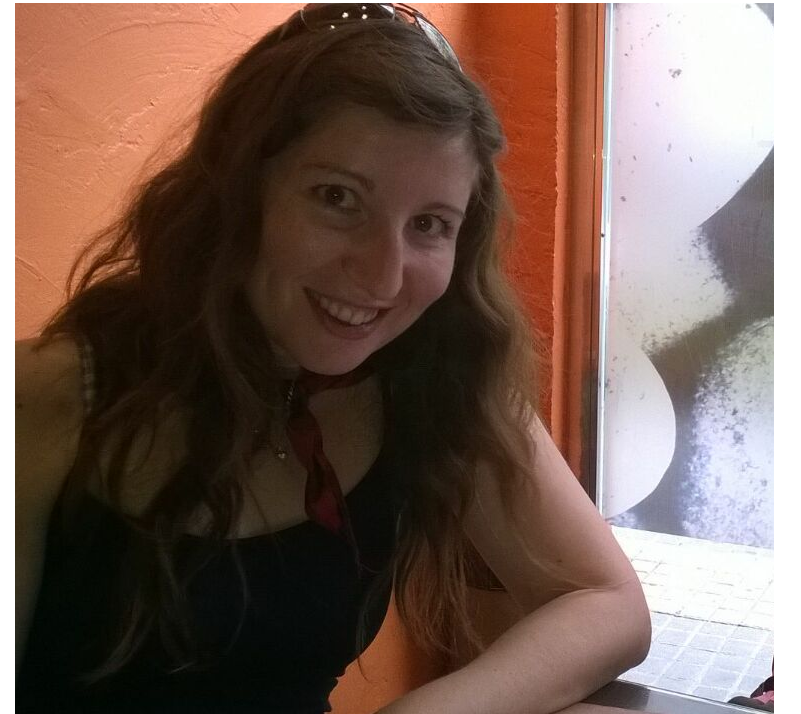
\includegraphics[scale=0.29]{maria.png}\\
    María José Peláez Montalvo\\ 
    {\small Coordinadora Revista Soluçoes}\\
    \vspace{1pt}
    %\vspace{0.1\textheight}
  \end{figurebox}
\vspace{1cm}
  La creación de esta revista lleva varias etapas, una primera etapa
  de discusión, de selección de temas por el equipo. Una etapa de
  estudio, de búsqueda de información y de creación. Una tercera etapa
  de revisión y discusión. Una cuarta etapa de maquetación. Una etapa
  de revisión final y llega el momento culminante: la impresión de la
  revista. En paralelo vamos subiendo los contenidos al formato
  digital donde os damos más informaciones, como son \emph{aplicaciones web}
  diseñada por nosotros para que podáis jugar con los conceptos o
  usarlas para enseñarlas a otros y los \emph{códigos} de los programas y
  gráficos expuestos en la revista. Y la etapa final es que llegue a
  vosotros y la recibáis, como me han contado, con una sonrisa.

 Nos gustaría que nos escribiéseis más, que
  nos contéis de que os encantaría os hablásemos, que temas os parece
  de interés, que inquietudes tenéis y si conocéis novedades que
  mencionar mandárnoslo. Estamos abiertos y felices de poder conoceros
  e intentad daros mediante nuestra revista una infinita satisfacción
  de amor a la ciencia.

  Aprovecho para desearos un feliz 2015 en nombre de todo mi
  equipo. Sigan soñando y recordando que una gran aportación no es
  sino una suma de pequeñas aportaciones.


\end{multicols}
\vspace{2cm}
      \centering
  
\includegraphics[scale=0.8]{pubmm.png}\\
 \newpage
%%% Local Variables: 
%%% mode: latex
%%% TeX-master: "nadaesimposible"
%%% End: 


